\chapter{DataSource V2 and Extensions}
\label{ch:dsv2}

\begin{chapterintro}
Iceberg is not built into Spark. It plugs in through the DataSource V2 API, and the
planner negotiates with it: which filters can you apply, which columns do you need,
can you answer this aggregate yourself? Understanding that negotiation explains why
some predicates prune and others do not, and why some \texttt{COUNT(*)} queries take
a tenth of a second on 30~million rows. This chapter reads the contract from the
outside --- through the interfaces Iceberg's classes implement, through what the
plan shows for thirteen different \texttt{WHERE} clauses, through the statistics the
source reports, and through what happens to a write when a task fails --- and then
shows how a jar adds Catalyst rules and SQL syntax to a session. Every output comes
from the lab in \Cref{sec:refenv-lab} (Spark 3.5.2, Iceberg 1.6.1).
\end{chapterintro}

\section{The DataSource V2 read and write API}
\label{sec:dsv2-api}

DataSource V2 (DSv2) is the interface contract between Catalyst and an external
table source. Rather than describe it in the abstract, the lab asked the live
objects which interfaces they implement (\Cref{tab:dsv2-interfaces}). A source is
a stack of four objects --- catalog, table, scan builder, scan --- and each
interface a class implements is a capability the planner may use.

\begin{table}[htbp]
\centering\footnotesize
\renewcommand{\arraystretch}{1.2}
\begin{tabular}{@{}p{1.9cm}p{5.8cm}p{6.5cm}@{}}
\toprule
\textbf{Object} & \textbf{Interface (Spark 3.5)} & \textbf{What it lets the planner do, and where this book shows it} \\
\midrule
catalog & \texttt{TableCatalog}, \texttt{SupportsNamespaces} & resolve \texttt{lab.db.orders} to a table (\Cref{ch:catalogs}) \\
 & \texttt{ProcedureCatalog} & \texttt{CALL lab.system.rewrite\_data\_files(...)} (\Cref{sec:dsv2-extensions}) \\
 & \texttt{StagingTableCatalog} & stage a table so a failed \texttt{CREATE TABLE AS SELECT} leaves nothing (claim --- not tested) \\
 & \texttt{FunctionCatalog} & \texttt{bucket}, \texttt{days} and the other partition transforms as functions \\
table & \texttt{SupportsRead}, \texttt{SupportsWrite} & obtain a scan builder or a write builder (this section) \\
 & \texttt{SupportsDeleteV2} & a \texttt{DELETE} on a whole partition resolved from metadata (\Cref{ch:iceberg-write}) \\
 & \texttt{SupportsRowLevelOperations} & \texttt{UPDATE}, \texttt{DELETE}, \texttt{MERGE} as copy-on-write or merge-on-read (\Cref{ch:iceberg-write}) \\
 & \texttt{SupportsMetadataColumns} & the hidden \texttt{\_file} and \texttt{\_pos} columns \\
scan builder & \texttt{SupportsPushDownV2Filters} & the filter negotiation (\Cref{sec:dsv2-pushdown}) \\
 & \texttt{SupportsPushDownRequiredColumns} & column pruning (\Cref{sec:pruning-column}) \\
 & \texttt{SupportsPushDownAggregates} & \texttt{COUNT}, \texttt{MIN}, \texttt{MAX} from metadata (\Cref{fig:aggregate-pushdown}) \\
 & \texttt{SupportsReportStatistics} & the size estimate behind join selection (\Cref{sec:dsv2-splits-stats}) \\
scan & \texttt{SupportsReportPartitioning} & storage-partitioned joins (\Cref{sec:joins-spj}) \\
 & \texttt{SupportsRuntimeV2Filtering} & dynamic partition pruning (\Cref{sec:pruning-dpp}) \\
\bottomrule
\end{tabular}
\caption{The DSv2 interfaces implemented by Iceberg 1.6.1's \texttt{SparkCatalog},
\texttt{SparkTable}, \texttt{SparkScanBuilder} and \texttt{SparkBatchQueryScan}, read by
reflection from a running session. Each row is a capability the planner can use,
and each chapter that shows its effect is cited.}
\label{tab:dsv2-interfaces}
\end{table}

For a read, a \texttt{TableProvider} resolves a table name to a \texttt{Table},
which hands back a \texttt{ScanBuilder} the planner negotiates with
(\Cref{sec:dsv2-pushdown}) before it ever produces a physical scan. For a write,
the same \texttt{Table} hands back a \texttt{WriteBuilder}, and the write is a
fixed sequence of hops: the \texttt{WriteBuilder} produces a \texttt{BatchWrite}
on the driver, which ships a \texttt{DataWriterFactory} to the executors; each task
gets a \texttt{DataWriter}, writes its partition, and returns a small
\texttt{WriterCommitMessage} (for Iceberg, the list of files it wrote); only when
\emph{every} message has arrived does the driver call \texttt{BatchWrite.commit()}
once. That single call is the DSv2 hook behind Iceberg's atomic pointer swap
(\Cref{sec:cat-swap}); \Cref{fig:dsv2-write-protocol} draws the sequence and the
failure path.

\begin{figure}[htbp]
  \centering
  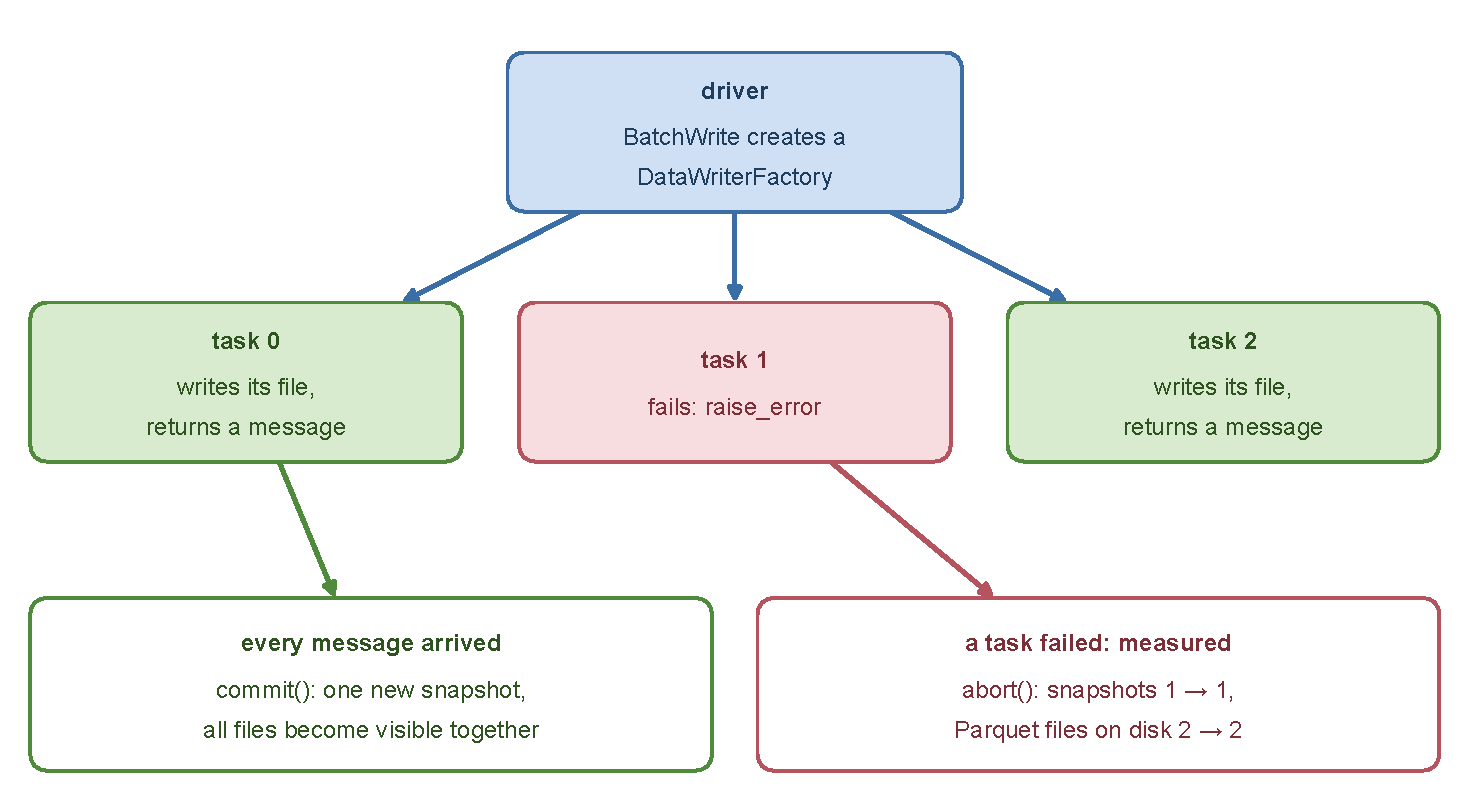
\includegraphics[width=0.9\linewidth]{dsv2-write-protocol.pdf}
  \caption{The write protocol, with the failure path measured. A task that raises an
  error stops the job before \texttt{commit()}: the table had one snapshot and two
  data files before the failed \texttt{INSERT} and the same afterwards.}
  \label{fig:dsv2-write-protocol}
\end{figure}

The lab checked the failure path directly. An \texttt{INSERT} whose last tasks
evaluate \texttt{raise\_error('boom at the end')} aborted the job; the table had
\textbf{1 snapshot and 2 Parquet files} on disk before and the same after. Tasks
that had already finished writing their files did not leave them behind: the
\texttt{abort} call cleans them up. A reader therefore never sees a partial write,
and a failed job costs disk only until the abort runs. (When the JVM dies before it
can abort --- a killed driver --- files can remain; those are the orphans of
\Cref{sec:ice-write-expiration}.)

\section{Pushdown negotiation}
\label{sec:dsv2-pushdown}

Pushdown under DSv2 is a negotiation, not a guarantee: the planner offers a source
a set of filters, columns, and (since Spark 3.2, for a narrow set of cases)
aggregates, and the source reports back which it can apply. Iceberg implements the
\emph{V2} filter interface, \texttt{SupportsPushDownV2Filters}, and its reply has
more than two outcomes. The lab ran thirteen \texttt{WHERE} shapes against the
30-million-row \texttt{orders} table and recorded, for each, how many rows left the
scan and whether Spark kept a \texttt{Filter} node above it
(\Cref{fig:pushdown-rows-by-predicate}).

\begin{figure}[htbp]
  \centering
  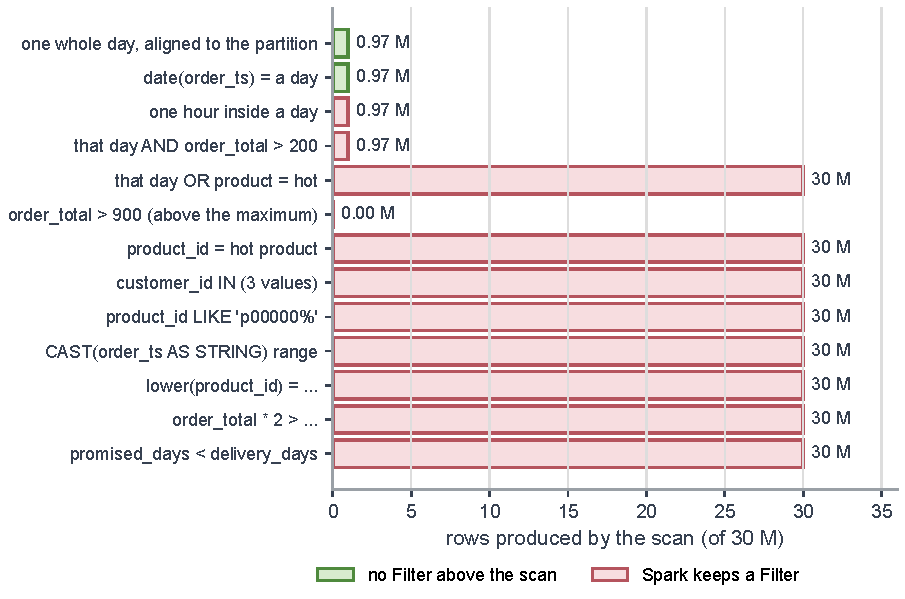
\includegraphics[width=\linewidth]{pushdown-rows-by-predicate.pdf}
  \caption{Rows produced by the scan for thirteen predicates. Only two --- a range
  that equals exactly one day partition, and the \texttt{date()} form that Iceberg
  rewrites to that range --- leave no \texttt{Filter} above the scan. Every other
  predicate keeps one.}
  \label{fig:pushdown-rows-by-predicate}
\end{figure}

Three things are visible. First, there are three outcomes, not two
(\Cref{fig:dsv2-pushdown-negotiation}). A predicate that coincides with the
partition boundary is \emph{fully handled}: the scan yields exactly the day's
967,939 rows and no \texttt{Filter} remains. A predicate on a data column is
\emph{pushed to prune files and row groups} but Iceberg does not filter rows
itself, so Spark keeps its \texttt{Filter}; whether the pushdown saved anything
depends on the data layout. And a predicate Iceberg cannot translate --- a
\texttt{CAST} to string, a function, arithmetic --- is \emph{not pushed} at all.

\begin{figure}[htbp]
  \centering
  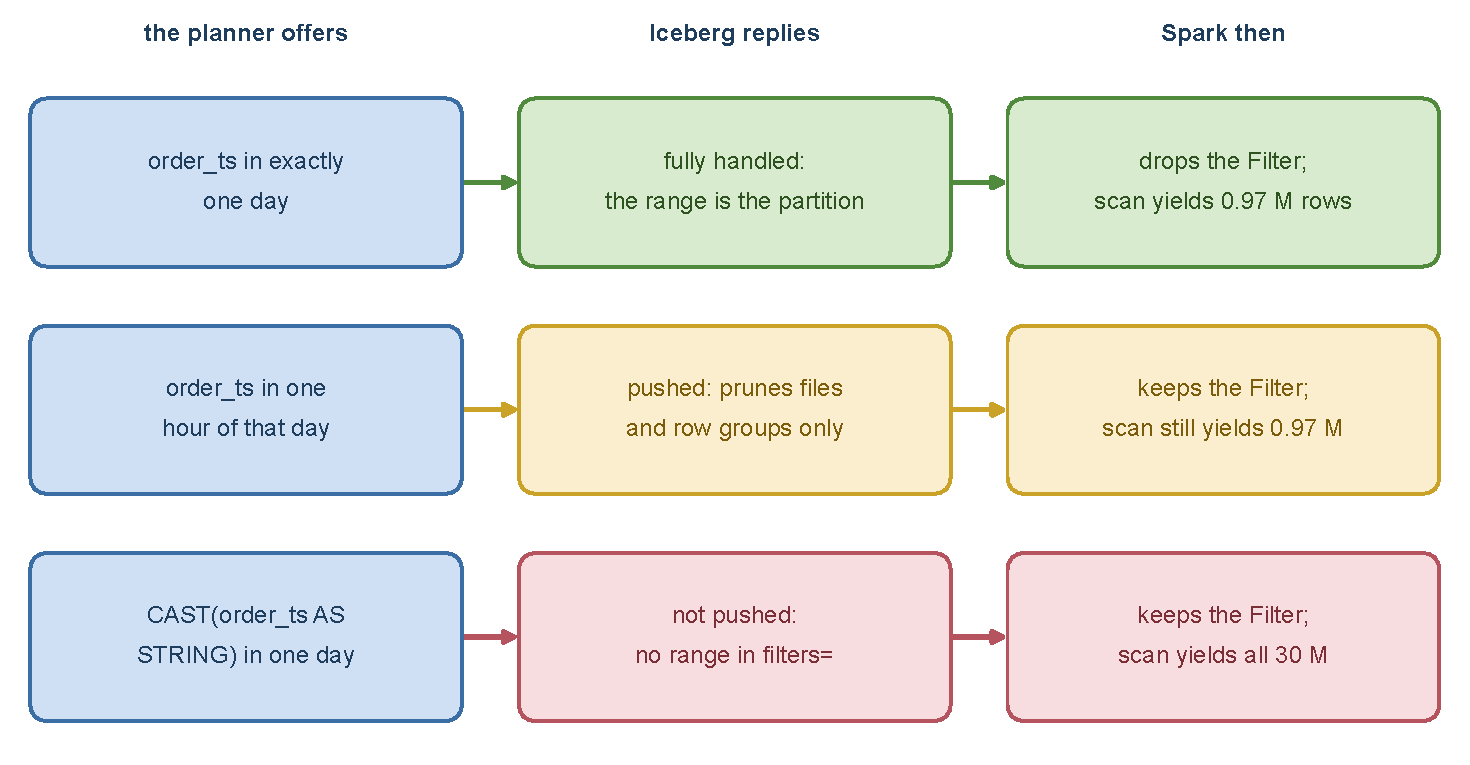
\includegraphics[width=0.9\linewidth]{dsv2-pushdown-negotiation.pdf}
  \caption{The same negotiation, three outcomes. Only a predicate that equals the
  partition boundary is fully handled; one hour inside the partition is pushed for
  pruning but re-checked by Spark; a \texttt{CAST} is not pushed.}
  \label{fig:dsv2-pushdown-negotiation}
\end{figure}

Second, \emph{pushed} does not mean \emph{pruned}. \texttt{product\_id = 'p0000042'}
appears in the scan's \texttt{filters=} list, yet the scan produced all 30~million
rows: the hot product is 30\% of the data and appears in every file, so no file's
statistics can exclude it. \texttt{order\_total > 900} is the opposite case: the
column's maximum is 305, so file statistics eliminated every file and the scan
produced \textbf{zero} rows --- while Spark still kept a \texttt{Filter} above it.
The same pushed filter is worthless or decisive depending on whether the column's
value ranges separate the files, which is the argument of \Cref{ch:iceberg-layout}.

Third, the way a predicate is written decides its outcome. The listing shows the
scan nodes for the three cases of \Cref{fig:dsv2-pushdown-negotiation}, copied from
the plans (the \texttt{filters=} list is where the negotiation's answer is
visible):

\begin{lstlisting}[language=text,style=plan,caption={The scan node shows what Iceberg accepted (\texttt{filters=}); lines shortened},captionpos=b,label=lst:dsv2-scan-lines]
-- one whole day (aligned)
BatchScan lab.db.orders[order_ts, order_total] [filters=order_ts IS NOT NULL,
  order_ts >= 1772668800000000, order_ts < 1772755200000000, groupedBy=]
-- one hour inside that day  (a Filter node remains above the scan)
BatchScan lab.db.orders[order_ts, order_total] [filters=order_ts IS NOT NULL,
  order_ts >= 1772704800000000, order_ts < 1772708400000000, groupedBy=]
-- CAST(order_ts AS STRING) in one day  (no range was pushed)
BatchScan lab.db.orders[order_ts, order_total] [filters=order_ts IS NOT NULL, groupedBy=]
\end{lstlisting}

\texttt{SupportsPushDownRequiredColumns} is the same negotiation for columns: the
first line of each scan node above lists only \texttt{order\_ts} and
\texttt{order\_total}, the two columns the query uses.

\paragraph{Aggregate pushdown.} \texttt{SupportsPushDownAggregates} lets Iceberg
answer some aggregates from manifest metadata without opening a data file. The
lab ran six aggregates (\Cref{fig:aggregate-pushdown}); the plan root tells which
path was taken: a \texttt{LocalTableScan} means the answer was already computed.

\begin{figure}[htbp]
  \centering
  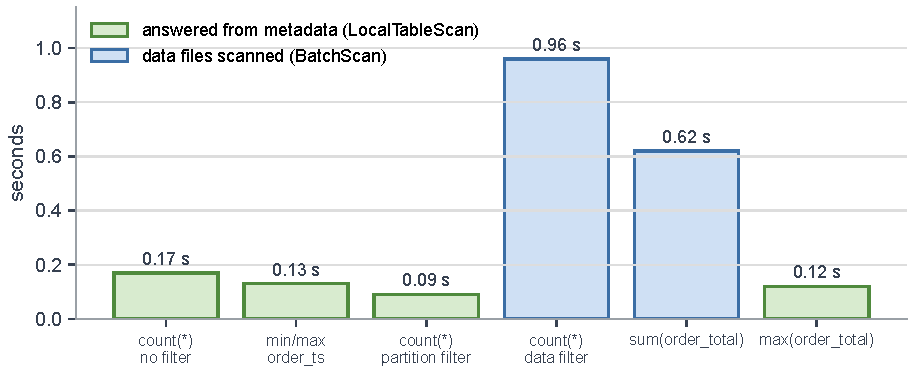
\includegraphics[width=\linewidth]{aggregate-pushdown.pdf}
  \caption{\texttt{COUNT(*)} on the whole table, on one day, \texttt{MIN}/\texttt{MAX}
  of \texttt{order\_ts} and \texttt{MAX(order\_total)} were answered from metadata in
  0.09--0.17~s. \texttt{COUNT(*)} with a data-column filter and \texttt{SUM} had to
  scan the data files (0.6--1.0~s).}
  \label{fig:aggregate-pushdown}
\end{figure}

The rule follows from what the manifests record. Each data file's entry carries its
record count and, per column, a lower and upper bound; a table-wide \texttt{COUNT},
\texttt{MIN} or \texttt{MAX} is a combination of those numbers. A \texttt{SUM}
needs the values; a \texttt{COUNT} filtered on a data column needs to know which
rows match. Pushing the aggregate is also the reason why a \texttt{COUNT(*)} on a
30-million-row table is not a useful benchmark of scan speed: it never scans.

\section{How Iceberg reports splits and statistics}
\label{sec:dsv2-splits-stats}

A DSv2 source does not hand the planner data directly. It hands back a set of
\texttt{InputPartition}s (Iceberg's version of the split planning of
\Cref{sec:ice-read-splits}) and a \texttt{PartitionReaderFactory} that reads each
one. Separately, \texttt{SupportsReportStatistics} tells the planner an estimated
size and row count \emph{before} the scan runs. The lab printed what the
optimizer saw (\Cref{tab:dsv2-stats}).

\begin{table}[htbp]
\centering\footnotesize
\renewcommand{\arraystretch}{1.2}
\begin{tabular}{@{}p{5.3cm}rrr@{}}
\toprule
\textbf{Scan} & \textbf{sizeInBytes} & \textbf{rowCount} & \textbf{bytes per row} \\
\midrule
\texttt{orders}, all 7 columns & 2,520,000,000 & 30,000,000 & 84 \\
\texttt{orders}, one day (partition-pruned) & 81,306,876 & 967,939 & 84 \\
\texttt{orders}, \texttt{product\_id = hot} & 2,520,000,000 & none & --- \\
\texttt{dim\_product}, all 6 columns & 216,000,000 & 2,000,000 & 108 \\
\texttt{dim\_date}, all 4 columns & 11,680 & 365 & 32 \\
\bottomrule
\end{tabular}
\caption{What \texttt{SupportsReportStatistics} reported to the optimizer. The
per-row figure is the same for every row count, and the data-column filter changed
nothing --- the source has no selectivity information.}
\label{tab:dsv2-stats}
\end{table}

Three facts follow. The estimate is built from record counts, not from file bytes:
a table of exactly the same bytes but fewer records would report less. It does
respond to \emph{partition pruning}: the one-day scan reports 81~MB because the
manifest list narrowed it before the estimate was taken, which is why a
tightly pruned scan of a huge table can legitimately report itself as small. And it
ignores a data-column predicate: \texttt{product\_id = hot} reports the full 2.52~GB
with an unknown row count, because Iceberg has no histogram to estimate
selectivity from. The per-row figures are not arbitrary: 84, 108 and 32 are the sums
of Spark's default widths for the columns' types (strings 20 bytes, doubles and
timestamps 8, integers and dates 4), so the estimate is \emph{rows times a width
derived from the schema}, not a measurement of Parquet bytes. That is why
\conf{spark.sql.autoBroadcastJoinThreshold} compares an uncompressed estimate
(\Cref{ch:aqe}) and why \texttt{dim\_product}, which occupies about 170~MB on disk,
is reported as 216~MB.

\section{Custom Catalyst rules and SQL extensions}
\label{sec:dsv2-extensions}

Nothing about this negotiation requires modifying Spark itself. A
\texttt{SparkSessionExtensions} entry point lets an external jar register
additional Catalyst rules --- injected into the analyzer, the optimizer, or physical
planning, alongside Spark's own rules from \Cref{sec:catalyst-rules} --- as well as
entirely new SQL syntax the parser would not otherwise recognize. Iceberg's
\texttt{IcebergSparkSessionExtensions} is exactly this mechanism, and the lab shows
what it adds by taking it away. The same four statements were run in a session with
\conf{spark.sql.extensions} empty (\Cref{tab:dsv2-noext}).

\begin{table}[htbp]
\centering\footnotesize
\renewcommand{\arraystretch}{1.2}
\begin{tabular}{@{}p{5.4cm}p{8.8cm}@{}}
\toprule
\textbf{Statement, no extension registered} & \textbf{Result} \\
\midrule
\texttt{CALL lab.system.rewrite\_data\_files(...)} & \texttt{PARSE\_SYNTAX\_ERROR: Syntax error at or near 'CALL'} \\
\texttt{ALTER TABLE orders ADD PARTITION FIELD ...} & \texttt{PARSE\_SYNTAX\_ERROR: Syntax error at or near 'FIELD'} \\
\texttt{SELECT count(*) FROM orders} & works \\
\texttt{SELECT count(*) FROM lab.db.orders.snapshots} & works \\
\bottomrule
\end{tabular}
\caption{With the extension removed, reads and metadata tables still work (they are
catalog and DSv2 features); the Iceberg-specific \emph{syntax} does not, because it
is parser rules the extension injects.}
\label{tab:dsv2-noext}
\end{table}

The split is the point. Reading, writing and metadata tables run on the catalog and
the DSv2 interfaces alone. \texttt{CALL} and \texttt{ADD PARTITION FIELD} are
grafted onto Spark's SQL grammar by the extension; none of it is native Spark SQL.
The compaction statement this book has used throughout is one such addition:

\begin{lstlisting}[language=SQL,caption={A procedure call, available only with the Iceberg extension registered},captionpos=b,label=lst:dsv2-call]
CALL lakehouse.system.rewrite_data_files(
  table => 'analytics.orders',
  strategy => 'binpack'
);
\end{lstlisting}

\section{Plugins}
\label{sec:dsv2-plugins}

Registering a catalog (\conf{spark.sql.catalog.<name>}, \Cref{sec:cat-spark-config})
and a session extension (\conf{spark.sql.extensions}) are both configuration keys
naming a class on the classpath. The lab's Iceberg installation is these two lines
plus the jar:

\begin{lstlisting}[language=bash,numbers=none,caption={The whole mechanism by which Iceberg is ``installed'' into a Spark session},captionpos=b,label=lst:dsv2-install]
spark.sql.catalog.lab=org.apache.iceberg.spark.SparkCatalog
spark.sql.extensions=org.apache.iceberg.spark.extensions.IcebergSparkSessionExtensions
\end{lstlisting}

The first key is what turns \texttt{lab.db.orders} into a resolvable name, by naming
the class that implements \texttt{TableCatalog} (\Cref{tab:dsv2-interfaces} lists
the seven interfaces that class implements); the second teaches the parser
\texttt{CALL}. No Spark source change, no rebuild. Any table format or connector
built to the same contracts plugs in the same way, which is the practical reason a
table format can evolve on its own release cadence independent of Spark's.

\begin{note}
Claim --- from the Spark 4 migration notes, not tested here: Spark 4.0 keeps the
DataSource V2 contract used above, but reorganizes parts of the extension API and
the default of \conf{spark.sql.ansi.enabled}. Re-run the thirteen-predicate
experiment on the Spark 4 Iceberg runtime before assuming the table in
\Cref{fig:pushdown-rows-by-predicate} carries over.
\end{note}

\section{From symptom to lever}
\label{sec:dsv2-levers}

\begin{table}[htbp]
\centering\footnotesize
\renewcommand{\arraystretch}{1.25}
\begin{tabular}{@{}p{3.1cm}p{3.7cm}p{4.1cm}p{3.2cm}@{}}
\toprule
\textbf{Symptom} & \textbf{Evidence} & \textbf{Lever} & \textbf{Cost} \\
\midrule
a filter does not reduce the data read & a \texttt{Filter} node above the scan; \texttt{filters=} lacks the predicate & rewrite so the column appears bare (no \texttt{CAST}, function or arithmetic) & none \\
a pushed filter still scans everything & \texttt{filters=} lists it but scan rows equal the table & sort or Z-order so the column's ranges separate files (\Cref{ch:iceberg-layout}) & a rewrite \\
a time-range filter leaves a \texttt{Filter} node & range does not align with the partition transform & accept it, or align the range to the transform & none \\
join strategy surprises & \texttt{EXPLAIN COST}: estimate far from disk size & remember: rows $\times$ default width; use a hint or statistics (\Cref{ch:joins}) & hint maintenance \\
\texttt{CALL} is a syntax error & \texttt{PARSE\_SYNTAX\_ERROR} at \texttt{CALL} & register \conf{spark.sql.extensions} & none \\
\bottomrule
\end{tabular}
\caption{The DSv2 levers: symptom, evidence, lever, cost.}
\label{tab:dsv2-levers}
\end{table}

\section{Summary}
\label{sec:dsv2-summary}

Iceberg is an ordinary DSv2 implementation from Spark's point of view: a catalog, a
table, a scan builder and a scan, each implementing the interfaces that unlock a
capability. The filter negotiation has three outcomes --- fully handled, pushed for
pruning only, not pushed --- and only a predicate that equals the partition boundary
is fully handled; the rest leave a \texttt{Filter} that re-checks every row.
Aggregates \texttt{COUNT}, \texttt{MIN} and \texttt{MAX} are answered from manifest
metadata in about a tenth of a second; \texttt{SUM} and data-filtered counts scan.
The statistics the source reports are rows times schema-derived widths, respond to
partition pruning, and ignore data-column predicates. A failed write leaves no
snapshot. And \texttt{CALL} and the DDL extensions exist only because a jar named in
\conf{spark.sql.extensions} added parser rules.

\exercisehead
\begin{exercises}
\item Write a query whose filter Iceberg fully handles and one whose filter is
      pushed but still leaves a \texttt{Filter} node. From the plan and the scan's
      row count, explain the difference.
\item Run \texttt{SELECT max(order\_total)} and \texttt{SELECT sum(order\_total)}
      on an Iceberg table. Which plan root appears for each, and what in the
      manifests explains it?
\item Print the interfaces a catalog, a table and a scan builder implement in your
      own session (the lab used reflection through \texttt{loadTable}) and match each
      to a behaviour of this chapter.
\end{exercises}
